\documentclass[twoside]{book}

% Packages required by doxygen
\usepackage{fixltx2e}
\usepackage{calc}
\usepackage{doxygen}
\usepackage[export]{adjustbox} % also loads graphicx
\usepackage{graphicx}
\usepackage[utf8]{inputenc}
\usepackage{makeidx}
\usepackage{multicol}
\usepackage{multirow}
\PassOptionsToPackage{warn}{textcomp}
\usepackage{textcomp}
\usepackage[nointegrals]{wasysym}
\usepackage[table]{xcolor}

% Font selection
\usepackage[T1]{fontenc}
\usepackage[scaled=.90]{helvet}
\usepackage{courier}
\usepackage{amssymb}
\usepackage{sectsty}
\renewcommand{\familydefault}{\sfdefault}
\allsectionsfont{%
  \fontseries{bc}\selectfont%
  \color{darkgray}%
}
\renewcommand{\DoxyLabelFont}{%
  \fontseries{bc}\selectfont%
  \color{darkgray}%
}
\newcommand{\+}{\discretionary{\mbox{\scriptsize$\hookleftarrow$}}{}{}}

% Page & text layout
\usepackage{geometry}
\geometry{%
  a4paper,%
  top=2.5cm,%
  bottom=2.5cm,%
  left=2.5cm,%
  right=2.5cm%
}
\tolerance=750
\hfuzz=15pt
\hbadness=750
\setlength{\emergencystretch}{15pt}
\setlength{\parindent}{0cm}
\setlength{\parskip}{3ex plus 2ex minus 2ex}
\makeatletter
\renewcommand{\paragraph}{%
  \@startsection{paragraph}{4}{0ex}{-1.0ex}{1.0ex}{%
    \normalfont\normalsize\bfseries\SS@parafont%
  }%
}
\renewcommand{\subparagraph}{%
  \@startsection{subparagraph}{5}{0ex}{-1.0ex}{1.0ex}{%
    \normalfont\normalsize\bfseries\SS@subparafont%
  }%
}
\makeatother

% Headers & footers
\usepackage{fancyhdr}
\pagestyle{fancyplain}
\fancyhead[LE]{\fancyplain{}{\bfseries\thepage}}
\fancyhead[CE]{\fancyplain{}{}}
\fancyhead[RE]{\fancyplain{}{\bfseries\leftmark}}
\fancyhead[LO]{\fancyplain{}{\bfseries\rightmark}}
\fancyhead[CO]{\fancyplain{}{}}
\fancyhead[RO]{\fancyplain{}{\bfseries\thepage}}
\fancyfoot[LE]{\fancyplain{}{}}
\fancyfoot[CE]{\fancyplain{}{}}
\fancyfoot[RE]{\fancyplain{}{\bfseries\scriptsize Generated by Doxygen }}
\fancyfoot[LO]{\fancyplain{}{\bfseries\scriptsize Generated by Doxygen }}
\fancyfoot[CO]{\fancyplain{}{}}
\fancyfoot[RO]{\fancyplain{}{}}
\renewcommand{\footrulewidth}{0.4pt}
\renewcommand{\chaptermark}[1]{%
  \markboth{#1}{}%
}
\renewcommand{\sectionmark}[1]{%
  \markright{\thesection\ #1}%
}

% Indices & bibliography
\usepackage{natbib}
\usepackage[titles]{tocloft}
\setcounter{tocdepth}{3}
\setcounter{secnumdepth}{5}
\makeindex

% Hyperlinks (required, but should be loaded last)
\usepackage{ifpdf}
\ifpdf
  \usepackage[pdftex,pagebackref=true]{hyperref}
\else
  \usepackage[ps2pdf,pagebackref=true]{hyperref}
\fi
\hypersetup{%
  colorlinks=true,%
  linkcolor=blue,%
  citecolor=blue,%
  unicode%
}

% Custom commands
\newcommand{\clearemptydoublepage}{%
  \newpage{\pagestyle{empty}\cleardoublepage}%
}

\usepackage{caption}
\captionsetup{labelsep=space,justification=centering,font={bf},singlelinecheck=off,skip=4pt,position=top}

%===== C O N T E N T S =====

\begin{document}

% Titlepage & ToC
\hypersetup{pageanchor=false,
             bookmarksnumbered=true,
             pdfencoding=unicode
            }
\pagenumbering{roman}
\begin{titlepage}
\vspace*{7cm}
\begin{center}%
{\Large My Project }\\
\vspace*{1cm}
{\large Generated by Doxygen 1.8.11}\\
\end{center}
\end{titlepage}
\clearemptydoublepage
\tableofcontents
\clearemptydoublepage
\pagenumbering{arabic}
\hypersetup{pageanchor=true}

%--- Begin generated contents ---
\chapter{Hierarchical Index}
\section{Class Hierarchy}
This inheritance list is sorted roughly, but not completely, alphabetically\+:\begin{DoxyCompactList}
\item \contentsline{section}{Fruit}{\pageref{classFruit}}{}
\begin{DoxyCompactList}
\item \contentsline{section}{Apple}{\pageref{classApple}}{}
\item \contentsline{section}{Grape}{\pageref{classGrape}}{}
\item \contentsline{section}{Orange}{\pageref{classOrange}}{}
\end{DoxyCompactList}
\item \contentsline{section}{List}{\pageref{classList}}{}
\item \contentsline{section}{List\+:\+:Node}{\pageref{structList_1_1Node}}{}
\end{DoxyCompactList}

\chapter{Class Index}
\section{Class List}
Here are the classes, structs, unions and interfaces with brief descriptions\+:\begin{DoxyCompactList}
\item\contentsline{section}{\hyperlink{structnode}{node} }{\pageref{structnode}}{}
\item\contentsline{section}{\hyperlink{structnode1}{node1} }{\pageref{structnode1}}{}
\item\contentsline{section}{\hyperlink{structnode__info}{node\+\_\+info} }{\pageref{structnode__info}}{}
\end{DoxyCompactList}

\chapter{File Index}
\section{File List}
Here is a list of all files with brief descriptions\+:\begin{DoxyCompactList}
\item\contentsline{section}{\hyperlink{Lab1_8c}{Lab1.\+c} }{\pageref{Lab1_8c}}{}
\end{DoxyCompactList}

\chapter{Class Documentation}
\hypertarget{classConcreteStrategyA}{}\section{Concrete\+StrategyA Class Reference}
\label{classConcreteStrategyA}\index{Concrete\+StrategyA@{Concrete\+StrategyA}}


Inheritance diagram for Concrete\+StrategyA\+:
\nopagebreak
\begin{figure}[H]
\begin{center}
\leavevmode
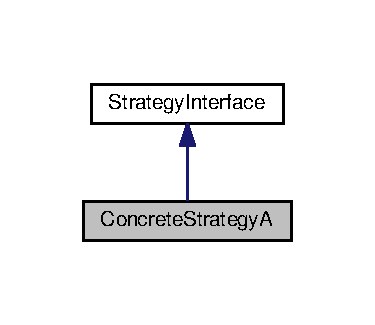
\includegraphics[width=180pt]{classConcreteStrategyA__inherit__graph}
\end{center}
\end{figure}


Collaboration diagram for Concrete\+StrategyA\+:
\nopagebreak
\begin{figure}[H]
\begin{center}
\leavevmode
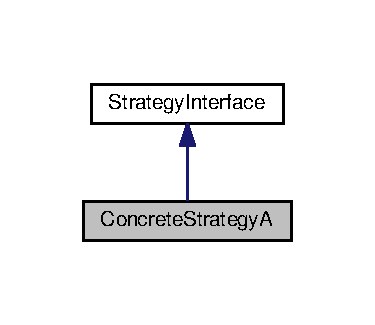
\includegraphics[width=180pt]{classConcreteStrategyA__coll__graph}
\end{center}
\end{figure}
\subsection*{Public Member Functions}
\begin{DoxyCompactItemize}
\item 
void \hyperlink{classConcreteStrategyA_aa9f7351ab4bfa87a2ccdef4e73813f10}{execute} () const override
\end{DoxyCompactItemize}


\subsection{Member Function Documentation}
\index{Concrete\+StrategyA@{Concrete\+StrategyA}!execute@{execute}}
\index{execute@{execute}!Concrete\+StrategyA@{Concrete\+StrategyA}}
\subsubsection[{\texorpdfstring{execute() const override}{execute() const override}}]{\setlength{\rightskip}{0pt plus 5cm}void Concrete\+Strategy\+A\+::execute (
\begin{DoxyParamCaption}
{}
\end{DoxyParamCaption}
) const\hspace{0.3cm}{\ttfamily [inline]}, {\ttfamily [override]}, {\ttfamily [virtual]}}\hypertarget{classConcreteStrategyA_aa9f7351ab4bfa87a2ccdef4e73813f10}{}\label{classConcreteStrategyA_aa9f7351ab4bfa87a2ccdef4e73813f10}


Implements \hyperlink{classStrategyInterface_a546e9e32a79d823262eb861919fd6653}{Strategy\+Interface}.


\begin{DoxyCode}
14         \{
15             cout << \textcolor{stringliteral}{"Called ConcreteStrategyA execute method"} << endl;
16         \}
\end{DoxyCode}


The documentation for this class was generated from the following file\+:\begin{DoxyCompactItemize}
\item 
\hyperlink{Strategy_8cpp}{Strategy.\+cpp}\end{DoxyCompactItemize}

\hypertarget{classConcreteStrategyB}{}\section{Concrete\+StrategyB Class Reference}
\label{classConcreteStrategyB}\index{Concrete\+StrategyB@{Concrete\+StrategyB}}


Inheritance diagram for Concrete\+StrategyB\+:
\nopagebreak
\begin{figure}[H]
\begin{center}
\leavevmode
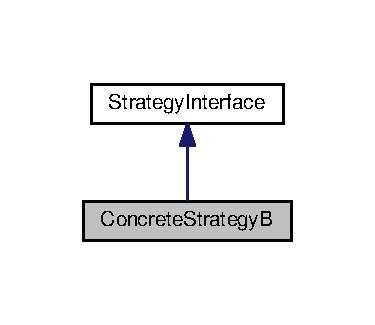
\includegraphics[width=180pt]{classConcreteStrategyB__inherit__graph}
\end{center}
\end{figure}


Collaboration diagram for Concrete\+StrategyB\+:
\nopagebreak
\begin{figure}[H]
\begin{center}
\leavevmode
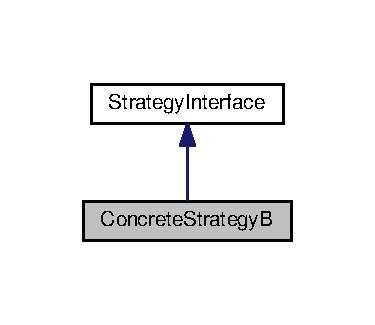
\includegraphics[width=180pt]{classConcreteStrategyB__coll__graph}
\end{center}
\end{figure}
\subsection*{Public Member Functions}
\begin{DoxyCompactItemize}
\item 
void \hyperlink{classConcreteStrategyB_ad17480f1a2bee9d7287954ffb5e040a2}{execute} () const override
\end{DoxyCompactItemize}


\subsection{Member Function Documentation}
\index{Concrete\+StrategyB@{Concrete\+StrategyB}!execute@{execute}}
\index{execute@{execute}!Concrete\+StrategyB@{Concrete\+StrategyB}}
\subsubsection[{\texorpdfstring{execute() const override}{execute() const override}}]{\setlength{\rightskip}{0pt plus 5cm}void Concrete\+Strategy\+B\+::execute (
\begin{DoxyParamCaption}
{}
\end{DoxyParamCaption}
) const\hspace{0.3cm}{\ttfamily [inline]}, {\ttfamily [override]}, {\ttfamily [virtual]}}\hypertarget{classConcreteStrategyB_ad17480f1a2bee9d7287954ffb5e040a2}{}\label{classConcreteStrategyB_ad17480f1a2bee9d7287954ffb5e040a2}


Implements \hyperlink{classStrategyInterface_a546e9e32a79d823262eb861919fd6653}{Strategy\+Interface}.


\begin{DoxyCode}
23         \{
24             cout << \textcolor{stringliteral}{"Called ConcreteStrategyB execute method"} << endl;
25         \}
\end{DoxyCode}


The documentation for this class was generated from the following file\+:\begin{DoxyCompactItemize}
\item 
\hyperlink{Strategy_8cpp}{Strategy.\+cpp}\end{DoxyCompactItemize}

\hypertarget{classConcreteStrategyC}{}\section{Concrete\+StrategyC Class Reference}
\label{classConcreteStrategyC}\index{Concrete\+StrategyC@{Concrete\+StrategyC}}


Inheritance diagram for Concrete\+StrategyC\+:
\nopagebreak
\begin{figure}[H]
\begin{center}
\leavevmode
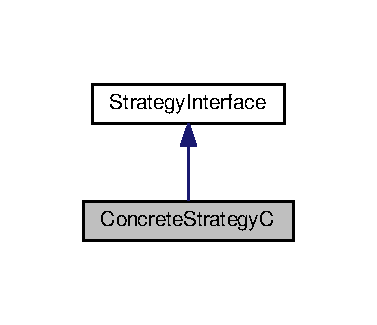
\includegraphics[width=181pt]{classConcreteStrategyC__inherit__graph}
\end{center}
\end{figure}


Collaboration diagram for Concrete\+StrategyC\+:
\nopagebreak
\begin{figure}[H]
\begin{center}
\leavevmode
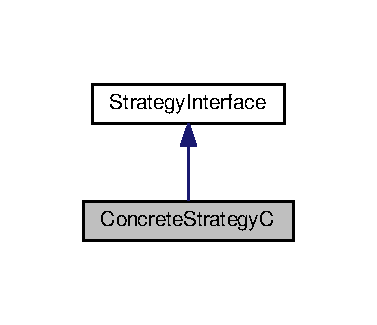
\includegraphics[width=181pt]{classConcreteStrategyC__coll__graph}
\end{center}
\end{figure}
\subsection*{Public Member Functions}
\begin{DoxyCompactItemize}
\item 
void \hyperlink{classConcreteStrategyC_a02c38120b6af81bfaa69d6a5f11c6fde}{execute} () const override
\end{DoxyCompactItemize}


\subsection{Member Function Documentation}
\index{Concrete\+StrategyC@{Concrete\+StrategyC}!execute@{execute}}
\index{execute@{execute}!Concrete\+StrategyC@{Concrete\+StrategyC}}
\subsubsection[{\texorpdfstring{execute() const override}{execute() const override}}]{\setlength{\rightskip}{0pt plus 5cm}void Concrete\+Strategy\+C\+::execute (
\begin{DoxyParamCaption}
{}
\end{DoxyParamCaption}
) const\hspace{0.3cm}{\ttfamily [inline]}, {\ttfamily [override]}, {\ttfamily [virtual]}}\hypertarget{classConcreteStrategyC_a02c38120b6af81bfaa69d6a5f11c6fde}{}\label{classConcreteStrategyC_a02c38120b6af81bfaa69d6a5f11c6fde}


Implements \hyperlink{classStrategyInterface_a546e9e32a79d823262eb861919fd6653}{Strategy\+Interface}.


\begin{DoxyCode}
32         \{
33             cout << \textcolor{stringliteral}{"Called ConcreteStrategyC execute method"} << endl;
34         \}
\end{DoxyCode}


The documentation for this class was generated from the following file\+:\begin{DoxyCompactItemize}
\item 
\hyperlink{Strategy_8cpp}{Strategy.\+cpp}\end{DoxyCompactItemize}

\hypertarget{classContext}{}\section{Context Class Reference}
\label{classContext}\index{Context@{Context}}


Collaboration diagram for Context\+:
\nopagebreak
\begin{figure}[H]
\begin{center}
\leavevmode
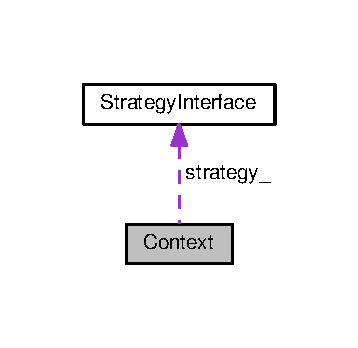
\includegraphics[width=172pt]{classContext__coll__graph}
\end{center}
\end{figure}
\subsection*{Public Member Functions}
\begin{DoxyCompactItemize}
\item 
\hyperlink{classContext_a4a38a1bd4ea50da0c91d8e5335467156}{Context} (\hyperlink{classStrategyInterface}{Strategy\+Interface} $\ast$strategy)
\item 
void \hyperlink{classContext_aac5a580be500769aac21a0d0a92ee902}{set\+\_\+strategy} (\hyperlink{classStrategyInterface}{Strategy\+Interface} $\ast$strategy)
\item 
void \hyperlink{classContext_a0f1e35fbff90abf753c54fbe5914805f}{execute} () const 
\end{DoxyCompactItemize}
\subsection*{Private Attributes}
\begin{DoxyCompactItemize}
\item 
\hyperlink{classStrategyInterface}{Strategy\+Interface} $\ast$ \hyperlink{classContext_afbfabe689b09b6558cd8b40c25a7d04b}{strategy\+\_\+}
\end{DoxyCompactItemize}


\subsection{Constructor \& Destructor Documentation}
\index{Context@{Context}!Context@{Context}}
\index{Context@{Context}!Context@{Context}}
\subsubsection[{\texorpdfstring{Context(\+Strategy\+Interface $\ast$strategy)}{Context(StrategyInterface *strategy)}}]{\setlength{\rightskip}{0pt plus 5cm}Context\+::\+Context (
\begin{DoxyParamCaption}
\item[{{\bf Strategy\+Interface} $\ast$}]{strategy}
\end{DoxyParamCaption}
)\hspace{0.3cm}{\ttfamily [inline]}, {\ttfamily [explicit]}}\hypertarget{classContext_a4a38a1bd4ea50da0c91d8e5335467156}{}\label{classContext_a4a38a1bd4ea50da0c91d8e5335467156}

\begin{DoxyCode}
43                                                      :\hyperlink{classContext_afbfabe689b09b6558cd8b40c25a7d04b}{strategy\_}(strategy)
44         \{
45         \}
\end{DoxyCode}


\subsection{Member Function Documentation}
\index{Context@{Context}!execute@{execute}}
\index{execute@{execute}!Context@{Context}}
\subsubsection[{\texorpdfstring{execute() const }{execute() const }}]{\setlength{\rightskip}{0pt plus 5cm}void Context\+::execute (
\begin{DoxyParamCaption}
{}
\end{DoxyParamCaption}
) const\hspace{0.3cm}{\ttfamily [inline]}}\hypertarget{classContext_a0f1e35fbff90abf753c54fbe5914805f}{}\label{classContext_a0f1e35fbff90abf753c54fbe5914805f}

\begin{DoxyCode}
53         \{
54             \hyperlink{classContext_afbfabe689b09b6558cd8b40c25a7d04b}{strategy\_}->\hyperlink{classStrategyInterface_a546e9e32a79d823262eb861919fd6653}{execute}();
55         \}
\end{DoxyCode}


Here is the call graph for this function\+:
\nopagebreak
\begin{figure}[H]
\begin{center}
\leavevmode
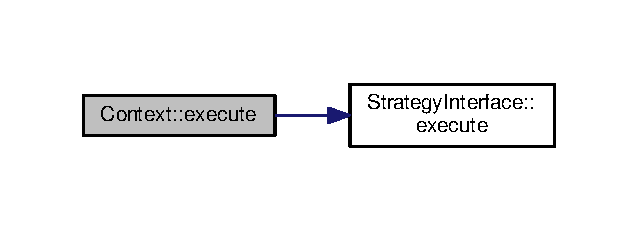
\includegraphics[width=306pt]{classContext_a0f1e35fbff90abf753c54fbe5914805f_cgraph}
\end{center}
\end{figure}


\index{Context@{Context}!set\+\_\+strategy@{set\+\_\+strategy}}
\index{set\+\_\+strategy@{set\+\_\+strategy}!Context@{Context}}
\subsubsection[{\texorpdfstring{set\+\_\+strategy(\+Strategy\+Interface $\ast$strategy)}{set_strategy(StrategyInterface *strategy)}}]{\setlength{\rightskip}{0pt plus 5cm}void Context\+::set\+\_\+strategy (
\begin{DoxyParamCaption}
\item[{{\bf Strategy\+Interface} $\ast$}]{strategy}
\end{DoxyParamCaption}
)\hspace{0.3cm}{\ttfamily [inline]}}\hypertarget{classContext_aac5a580be500769aac21a0d0a92ee902}{}\label{classContext_aac5a580be500769aac21a0d0a92ee902}

\begin{DoxyCode}
48         \{
49             \hyperlink{classContext_afbfabe689b09b6558cd8b40c25a7d04b}{strategy\_} = strategy;
50         \}
\end{DoxyCode}


\subsection{Member Data Documentation}
\index{Context@{Context}!strategy\+\_\+@{strategy\+\_\+}}
\index{strategy\+\_\+@{strategy\+\_\+}!Context@{Context}}
\subsubsection[{\texorpdfstring{strategy\+\_\+}{strategy_}}]{\setlength{\rightskip}{0pt plus 5cm}{\bf Strategy\+Interface}$\ast$ Context\+::strategy\+\_\+\hspace{0.3cm}{\ttfamily [private]}}\hypertarget{classContext_afbfabe689b09b6558cd8b40c25a7d04b}{}\label{classContext_afbfabe689b09b6558cd8b40c25a7d04b}


The documentation for this class was generated from the following file\+:\begin{DoxyCompactItemize}
\item 
\hyperlink{Strategy_8cpp}{Strategy.\+cpp}\end{DoxyCompactItemize}

\hypertarget{classStrategyInterface}{}\section{Strategy\+Interface Class Reference}
\label{classStrategyInterface}\index{Strategy\+Interface@{Strategy\+Interface}}


Inheritance diagram for Strategy\+Interface\+:
\nopagebreak
\begin{figure}[H]
\begin{center}
\leavevmode
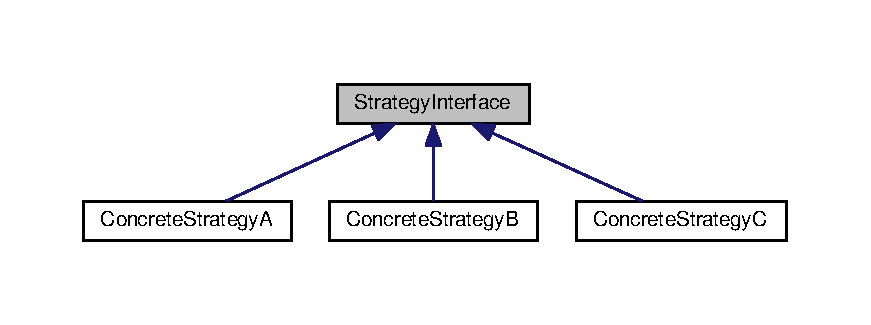
\includegraphics[width=350pt]{classStrategyInterface__inherit__graph}
\end{center}
\end{figure}
\subsection*{Public Member Functions}
\begin{DoxyCompactItemize}
\item 
virtual void \hyperlink{classStrategyInterface_a546e9e32a79d823262eb861919fd6653}{execute} () const =0
\end{DoxyCompactItemize}


\subsection{Member Function Documentation}
\index{Strategy\+Interface@{Strategy\+Interface}!execute@{execute}}
\index{execute@{execute}!Strategy\+Interface@{Strategy\+Interface}}
\subsubsection[{\texorpdfstring{execute() const =0}{execute() const =0}}]{\setlength{\rightskip}{0pt plus 5cm}virtual void Strategy\+Interface\+::execute (
\begin{DoxyParamCaption}
{}
\end{DoxyParamCaption}
) const\hspace{0.3cm}{\ttfamily [pure virtual]}}\hypertarget{classStrategyInterface_a546e9e32a79d823262eb861919fd6653}{}\label{classStrategyInterface_a546e9e32a79d823262eb861919fd6653}


Implemented in \hyperlink{classConcreteStrategyC_a02c38120b6af81bfaa69d6a5f11c6fde}{Concrete\+StrategyC}, \hyperlink{classConcreteStrategyB_ad17480f1a2bee9d7287954ffb5e040a2}{Concrete\+StrategyB}, and \hyperlink{classConcreteStrategyA_aa9f7351ab4bfa87a2ccdef4e73813f10}{Concrete\+StrategyA}.



The documentation for this class was generated from the following file\+:\begin{DoxyCompactItemize}
\item 
\hyperlink{Strategy_8cpp}{Strategy.\+cpp}\end{DoxyCompactItemize}

\chapter{File Documentation}
\hypertarget{Strategy_8cpp}{}\section{Strategy.\+cpp File Reference}
\label{Strategy_8cpp}\index{Strategy.\+cpp@{Strategy.\+cpp}}
{\ttfamily \#include $<$iostream$>$}\\*
Include dependency graph for Strategy.\+cpp\+:
\nopagebreak
\begin{figure}[H]
\begin{center}
\leavevmode
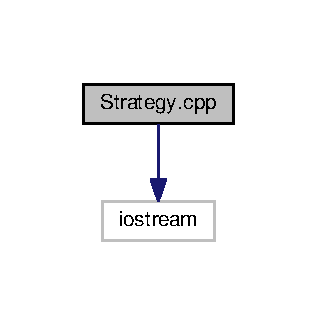
\includegraphics[width=152pt]{Strategy_8cpp__incl}
\end{center}
\end{figure}
\subsection*{Classes}
\begin{DoxyCompactItemize}
\item 
class \hyperlink{classStrategyInterface}{Strategy\+Interface}
\item 
class \hyperlink{classConcreteStrategyA}{Concrete\+StrategyA}
\item 
class \hyperlink{classConcreteStrategyB}{Concrete\+StrategyB}
\item 
class \hyperlink{classConcreteStrategyC}{Concrete\+StrategyC}
\item 
class \hyperlink{classContext}{Context}
\end{DoxyCompactItemize}
\subsection*{Functions}
\begin{DoxyCompactItemize}
\item 
int \hyperlink{Strategy_8cpp_a0ddf1224851353fc92bfbff6f499fa97}{main} (int argc, char $\ast$argv\mbox{[}$\,$\mbox{]})
\end{DoxyCompactItemize}


\subsection{Function Documentation}
\index{Strategy.\+cpp@{Strategy.\+cpp}!main@{main}}
\index{main@{main}!Strategy.\+cpp@{Strategy.\+cpp}}
\subsubsection[{\texorpdfstring{main(int argc, char $\ast$argv[])}{main(int argc, char *argv[])}}]{\setlength{\rightskip}{0pt plus 5cm}int main (
\begin{DoxyParamCaption}
\item[{int}]{argc, }
\item[{char $\ast$}]{argv\mbox{[}$\,$\mbox{]}}
\end{DoxyParamCaption}
)}\hypertarget{Strategy_8cpp_a0ddf1224851353fc92bfbff6f499fa97}{}\label{Strategy_8cpp_a0ddf1224851353fc92bfbff6f499fa97}

\begin{DoxyCode}
59 \{
60     \hyperlink{classConcreteStrategyA}{ConcreteStrategyA} concreteStrategyA;
61     \hyperlink{classConcreteStrategyB}{ConcreteStrategyB} concreteStrategyB;
62     \hyperlink{classConcreteStrategyC}{ConcreteStrategyC} concreteStrategyC;
63 
64     \hyperlink{classContext}{Context} contextA(&concreteStrategyA);
65     \hyperlink{classContext}{Context} contextB(&concreteStrategyB);
66     \hyperlink{classContext}{Context} contextC(&concreteStrategyC);
67 
68     contextA.execute(); \textcolor{comment}{// output: "Called ConcreteStrategyA execute method"}
69     contextB.execute(); \textcolor{comment}{// output: "Called ConcreteStrategyB execute method"}
70     contextC.execute(); \textcolor{comment}{// output: "Called ConcreteStrategyC execute method"}
71     
72     contextA.set\_strategy(&concreteStrategyB);
73     contextA.execute(); \textcolor{comment}{// output: "Called ConcreteStrategyB execute method"}
74     contextA.set\_strategy(&concreteStrategyC);
75     contextA.execute(); \textcolor{comment}{// output: "Called ConcreteStrategyC execute method"}
76 
77     \textcolor{keywordflow}{return} 0;
78 \}\end{DoxyCode}


Here is the call graph for this function\+:
\nopagebreak
\begin{figure}[H]
\begin{center}
\leavevmode
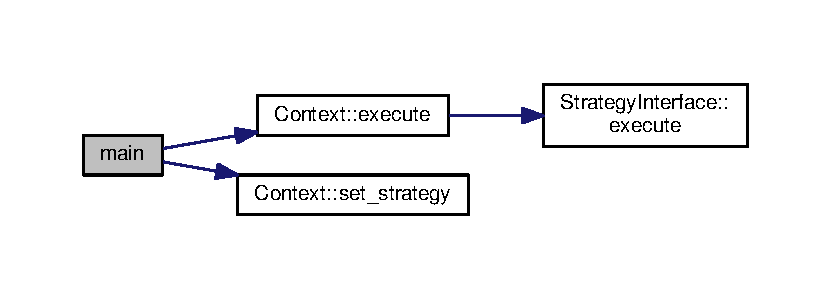
\includegraphics[width=350pt]{Strategy_8cpp_a0ddf1224851353fc92bfbff6f499fa97_cgraph}
\end{center}
\end{figure}



%--- End generated contents ---

% Index
\backmatter
\newpage
\phantomsection
\clearemptydoublepage
\addcontentsline{toc}{chapter}{Index}
\printindex

\end{document}
